\runningheader{Oppgave g), frivillig}{}{Side \thepage\ av \numpages}
% ********************************************************
% oppgave g) 
% ********************************************************  
\item
{\bf Effekten av støy ved numerisk derivasjon}
\label{oppg:g}

For å gjøre denne oppgaven må du gjort 
de frivillige oppgavene i~\ref{oppg:d}) og \ref{oppg:e}). 

Hensikten med oppgaven er å studere effekten av støy ved numerisk
integrasjon og derivasjon. Vi tar utgangspunkt i signalet fra
ligning~\eqref{eq:u2} hvor vi lager et signal uten støy som vi kaller
\fbox{\tt u1}, og et signal med støy som vi kaller \fbox{\tt u2}.

Vi benytter deretter Eulers forovermetode på begge signalene for å
beregne henholdsvis \fbox{\tt y1} og \fbox{\tt y2}.

I tillegg benytter vi bakoverderivasjon på begge signalene for å
beregne henholdsvis \fbox{\tt v1} og \fbox{\tt v2}.
For å studere effekten av metodevalg for derivasjon,
benytter vi senterderivasjon på signalet med støy og beregner \fbox{\tt v3}. 

\begin{itemize}
\item 
  Pass på at \fbox{\tt T\_s = 0.4} og kjør koden.
  Endre tidsskrittet i steg fra  \fbox{\tt T\_s = 0.4} til
  \fbox{\tt T\_s =  0.05}.
 Vi at du får et resultatet som ligner på figur~\ref{fig:fig1g_1}.
  Ta med figuren din i innleveringen.
 \begin{figure}[H]
      \centering
      \hspace*{0mm}\scalebox{0.43}{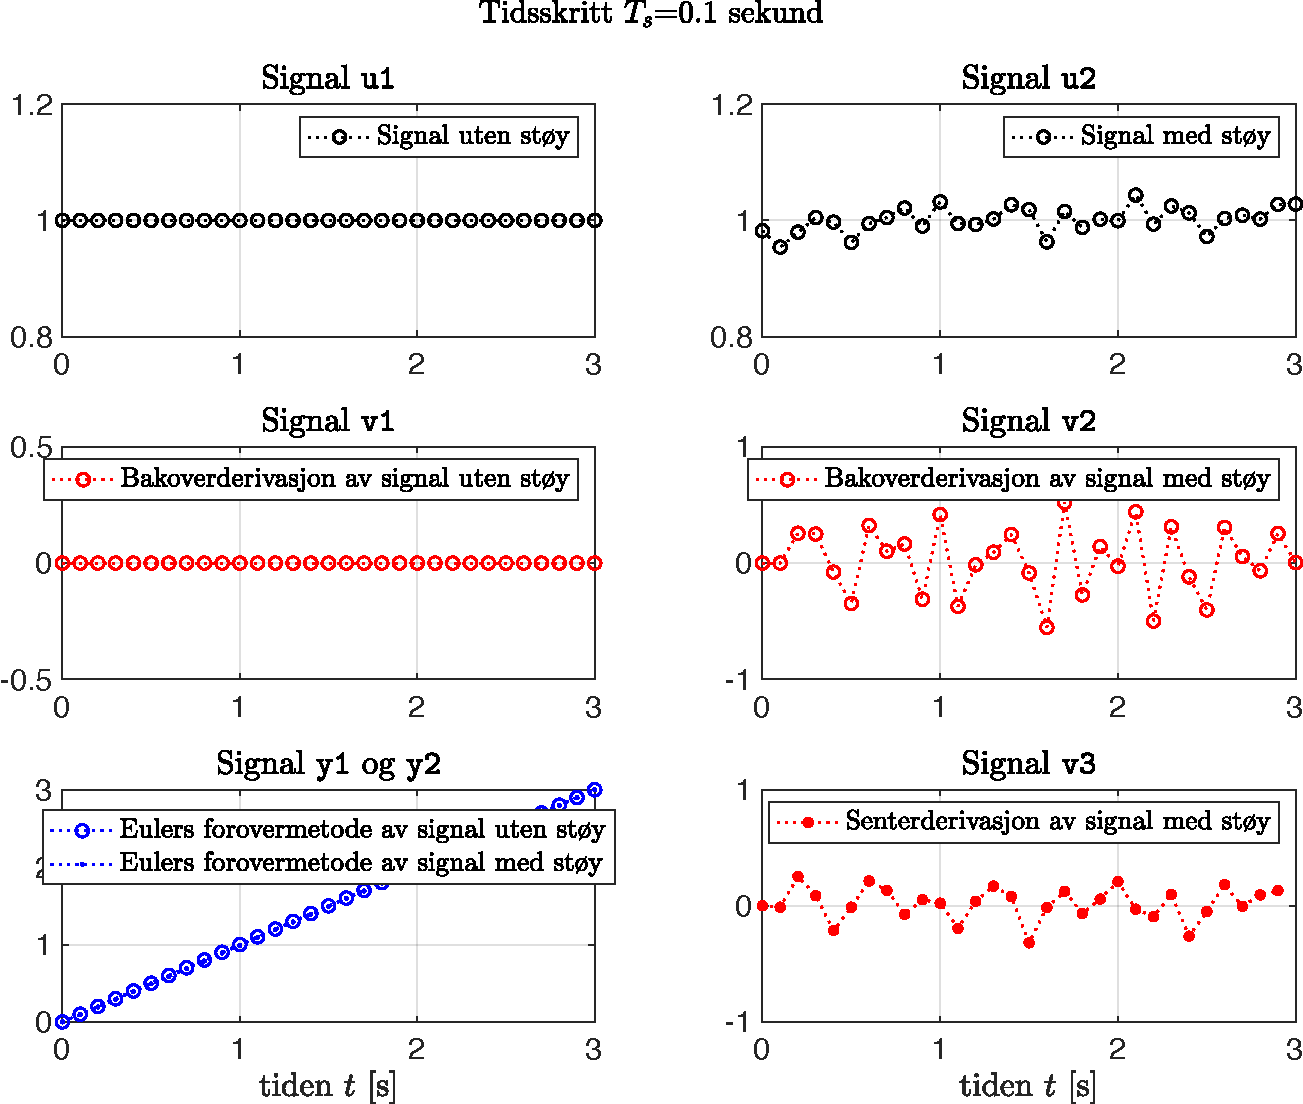
\includegraphics{fig3g_1.pdf}}
      \caption{Resultat som viser hvordan støy påvirker numerisk
        integrasjon og derivasjon.}
      \label{fig:fig1g_1}
    \end{figure}


\item  Hva skjer med signalene
  {\tt v2} og {\tt v3} etterhvert som tidsskrittet synker?
  Hva er forklaringen på at utslaget i
  disse to blir større og større?


\item Forklar hvorfor støy ikke påvirker numerisk
  integrasjon i særlig grad. 

\item Hva er grunnen til at senterderivasjon gir bedre resultat
  sammenlignet med bakoverderivasjon?
 
   
\end{itemize}

